\documentclass[10pt, a4paper, oneside]{article}
\usepackage[ngerman]{babel}
\usepackage{longtable}
\usepackage[shortlabels]{enumitem}

\usepackage{blindtext}
\usepackage{titlesec}
\usepackage{amsmath}
\usepackage[hidelinks]{hyperref}
\usepackage{parskip}
\usepackage{graphicx}
\usepackage{longtable}
\usepackage[shortlabels]{enumitem}
\usepackage{multirow}
\usepackage{nccmath}
\usepackage{rotating}
\usepackage{makecell}
\usepackage{multicol}
\usepackage{capt-of}
\usepackage{csquotes}
\usepackage{amsfonts}
\usepackage{caption}

\captionsetup[table]{position=bottom}

\titleformat{\section}
    {\normalfont\Large\bfseries}{}{0pt}{}

\let\oldsection\section
\renewcommand{\section}{
  \renewcommand{\theequation}{\thesection.\arabic{equation}}
  \oldsection}
\let\oldsubsection\subsection
\renewcommand{\subsection}{
  \renewcommand{\theequation}{\thesubsection.\arabic{equation}}
  \oldsubsection}

\makeatletter
\renewcommand{\maketitle}{
    \bgroup
    \centering
    \par\LARGE\@title  \\[20pt]
    \par\large\@author \\[10pt]
    \par\large\@date
    \par
    \egroup
}
\makeatother


\title{Technische Informatik\\[5pt]\Large{L\"osungen zum \"Ubungsblatt 01}\\[20pt]}
\author{Volodymyr But}
\date{WS24/25, FHS Trier}

% - - - - - - - - - - - - - - - - - - - - - - - - - - - - - - - - - - - - - - %

\begin{document}
\sloppy

\maketitle
\vspace{25px}

\section{Aufgabe 1}

In der Vorlesung wurde die sogenannte \textbf{Von-Neumann-Architektur}
vorgestellt. Erl"autern Sie den so genannten \textbf{Von-Neumann-Flaschenhals}.

\textbf{Erkl"arung}. Die Von-Neumann-Architektur besteht aus drei
Hauptkomponenten: dem Prozessor (CPU), dem Hauptspeicher und dem Bus. Der
Hauptspeicher speichert Daten und Programme, die vom Prozessor ausgeführt
werden. Der Bus verbindet den Prozessor mit dem Speicher. Das Problem bei dieser
Architektur besteht darin, dass sowohl Befehle als auch Daten nacheinander
geladen werden müssen, was zu einem Engpass in der Verbindung zwischen Prozessor
und Speicher führen kann. Die maximale Datenübertragungsrate wird also zwischen
Daten und Befehlen aufgeteilt, was als Von-Neumann-Flaschenhals bezeichnet wird.

\section{Aufgabe 2}

Welche alternative Architektur vermeidet den Von-Neumann-Flaschenhals?
Skizzieren Sie diese alternative Architektur?

\textbf{Erkl"arung}. Eine der alternativen Architekturen, die den
Von-Neumann-Flaschenhals vermeiden, ist die Harvard-Architektur. Sie teilt den
Hauptspeicher in zwei Bereiche auf: den Programmspeicher und den Datenspeicher.
Zusätzlich werden zwei separate Busse eingerichtet, die diese Speicher mit der
CPU verbinden. Dadurch wird eine gleichzeitige Übertragung von Daten und
Befehlen ermöglicht und der Von-Neumann-Flaschenhals vermieden.

\vspace{10px}
\begin{figure}[h]
    \centering
    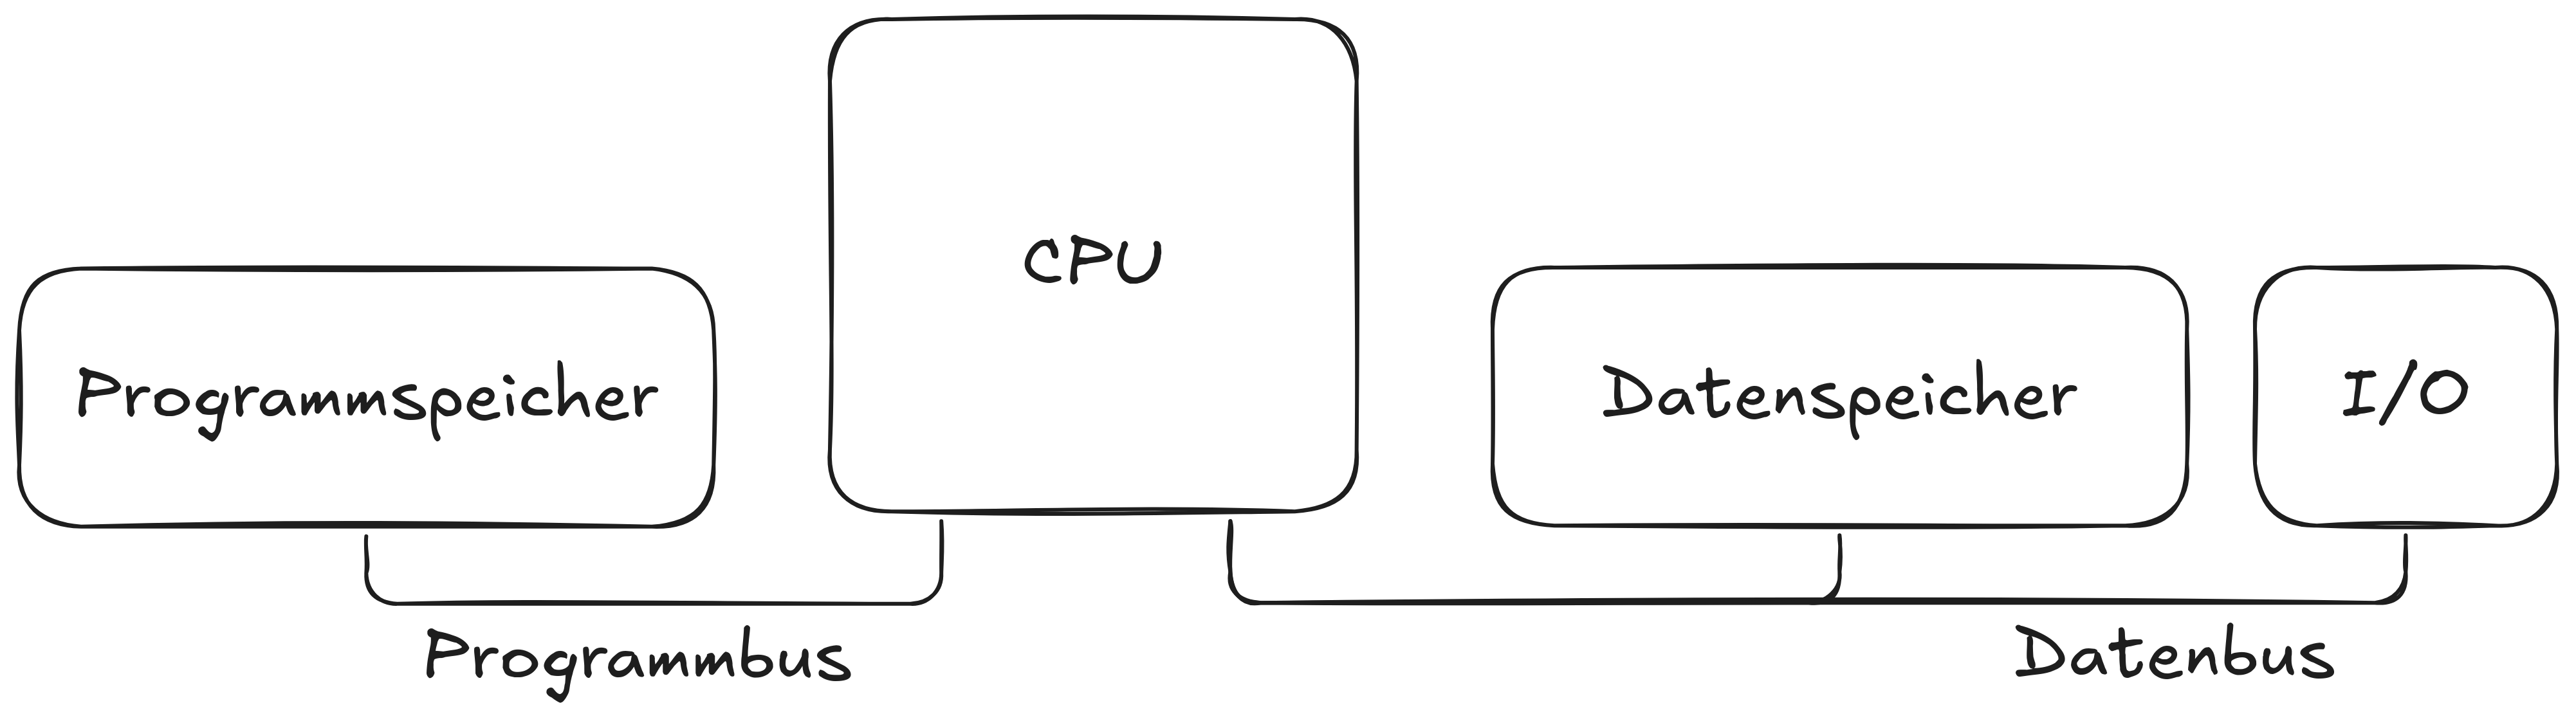
\includegraphics[width=1\textwidth]{./assets/harvard-architektur.png}
    \caption{Harvard-Architektur}
\end{figure}

\section{Aufgabe 3}

Erl"autern Sie die Unterschiede zwischen einer L/S-Architektur, einer
R/M-Architektur und einer R+M-Architektur.

\textbf{Erkl"arung}.

\begin{table}[h]
    \centering
    \begin{tabular}{p{0.33\linewidth}|p{0.33\linewidth}|p{0.33\linewidth}}
        L/S-Architektur & R/M-Architektur & R+M-Architektur \\
        \hline
        teilt die Befehle in zwei Kategorien ein: Speicherzugriff und
        ALU-Operationen. Dabei müssen sowohl Operanden als auch das Ergebnis
        einer Operation in Registern liegen &
        ermöglicht die Durchführung von Operationen im Speicher sowie in
        Registern. Bei diesem Ansatz kann sich einer der Operanden für
        Operationen im Speicher befinden, während der andere in einem Register
        liegt &
        wie bei der R/M-Architektur, mit der Ausnahme, dass zusätzlich alle
        Operanden im Speicher oder in Registern sein können
    \end{tabular}
    \caption{L/S- vs R/M- vs R+M-Architektur}
\end{table}

\section{Aufgabe 4}

In der Vorlesung wurde die Funktionsweise eines Relais erl"autert. Wird der
Schalter im Steuerkreis geschlossen, dann wird der Elektromagnet aktiviert und
schaltet mechanisch den Schalter des Lastkreis.

\begin{figure}[h]
    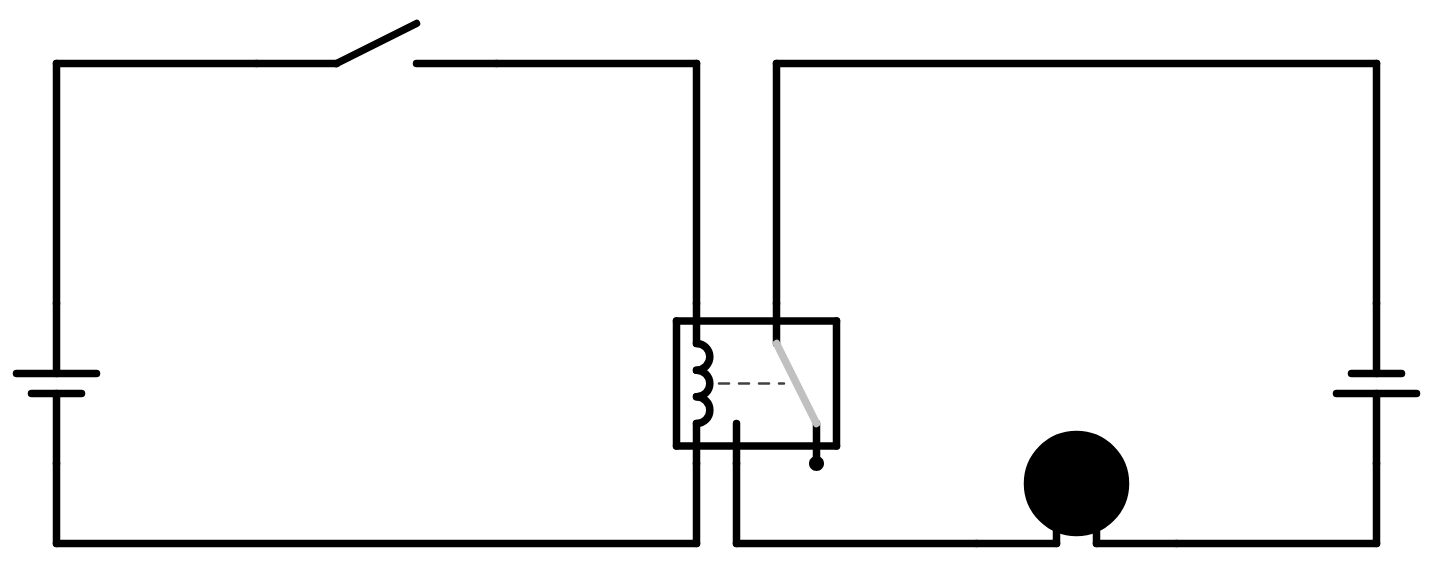
\includegraphics[width=1\textwidth]{./assets/relay-circuit.png}
    \caption{Das Relais}
\end{figure}

\pagebreak

\begin{enumerate}[(a)]
    \item Modifizieren Sie die Zeichnung bitte so, dass eine logische
        UND-Schaltung realisiert ist. Sie ben"otigen dazu zwei Schalter im
        Steuerkreis. Denken Sie z. B. an eine Hecken- schere oder eine
        Stanzmaschine, bei denen der Benutzer zwei Schalter dr"ucken muss um die
        Maschine zu bedienen.

        \textbf{L"osung:}

        \begin{figure}[h]
            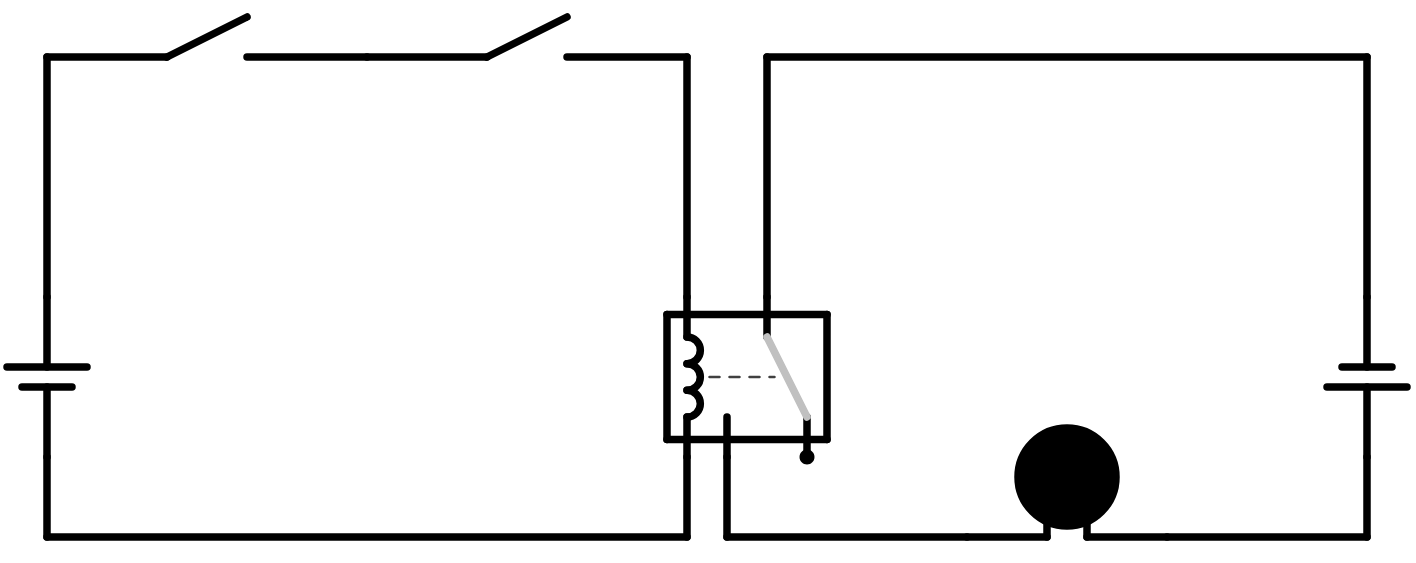
\includegraphics[width=1\textwidth]{./assets/und-circuit.png}
            \caption{UND-Schaltung}
        \end{figure}

    \item Modifizieren Sie die Zeichnung bitte so, dass eine logische ODER-Schaltung entsteht.
        Sie ben"otigen wieder Schalter im Steuerkreis. Denken Sie an den Notrufknopf
        von Patienten im Krankenhaus. Die rote Lampe im Schwesternzimmer
        (Lastkreis) erleuchtet wenn einer der Patienten den Schalter dr"uckt.

        \textbf{L"osung:}

        \begin{figure}[h]
            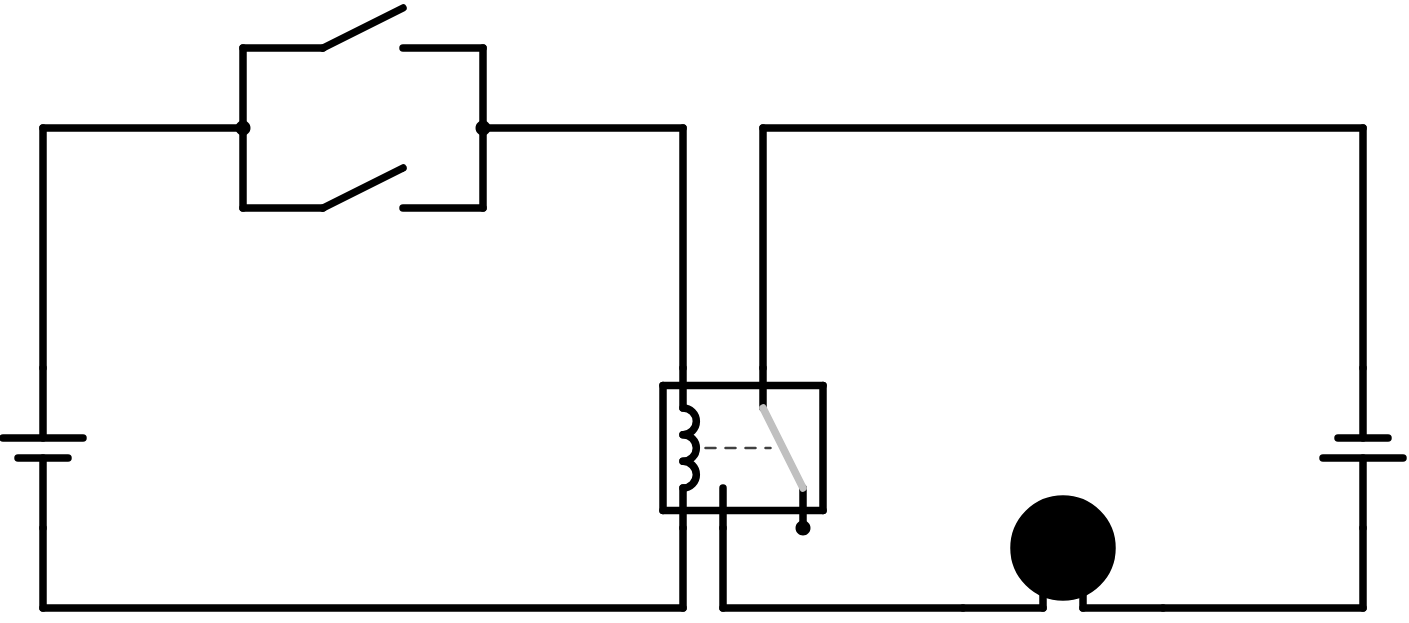
\includegraphics[width=1\textwidth]{./assets/oder-circuit.png}
            \caption{ODER-Schaltung}
        \end{figure}

    \item Modifizieren Sie die Zeichnung bitte so, dass eine logische
        NOT-Schaltung entsteht. Sie brauchen nur einen Schalter im Steuerkreis.
        Solange der Schalter geschaltet ist, bleibt die Maschine im Lastkreis
        aus. Wird der Schalter im Steuerkreis ge"offnet, l"auft die Maschine.
        Denken Sie z. B. an die Luftdruckbremse beim LKW. Solange Druck auf dem
        Kessel ist, bleibt die Bremsanlage unt"atig (Schalter im Steuerkreis
        geschlossen) und der LKW kann bewegt werden. Ohne Druck ist der
        Schalter offen und die Bremsanlage (Lastkreis) schaltet. Durch
        Bet"atigen des Bremspedals oder durch einen Defekt an der
        Luftdruckanlage w"urde der Schalter im Steuerkreis ge"offnet

        \textbf{L"osung:}

        \begin{figure}[h]
            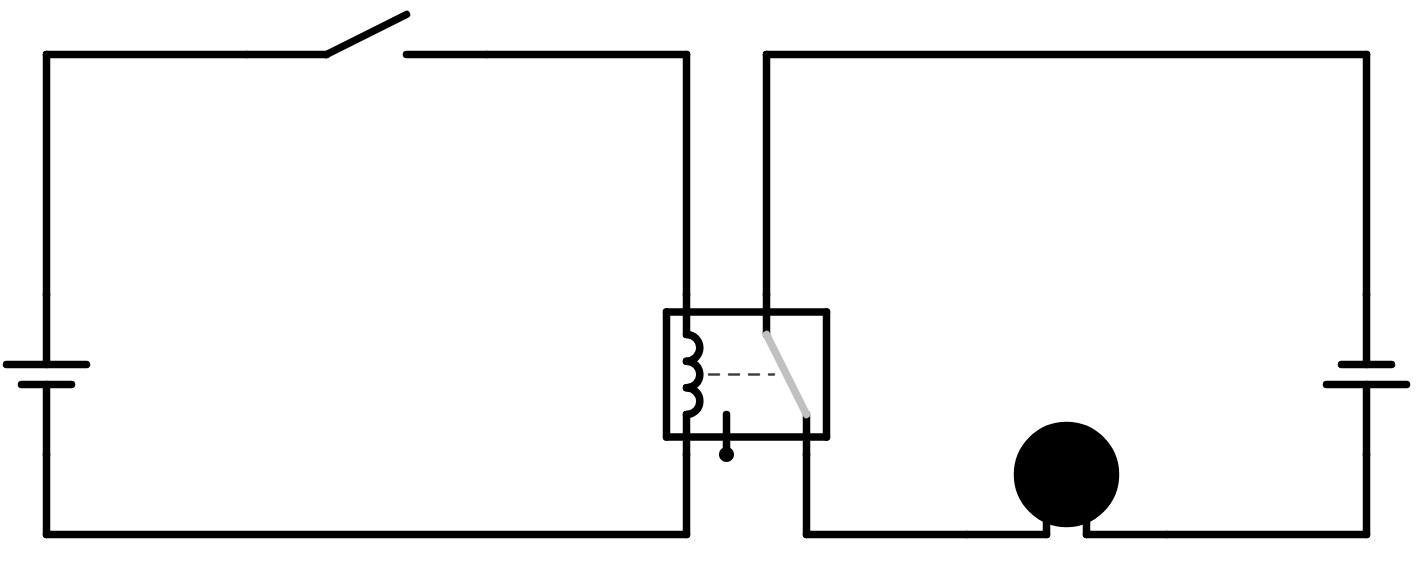
\includegraphics[width=1\textwidth]{./assets/not-circuit.png}
            \caption{NOT-Schaltung}
        \end{figure}

    \item Jetzt bauen Sie noch bitte eine Schaltung mit zwei Schaltern A und B
        im Steuerkreis, so dass die Maschine im Lastkreis l"auft, solange weder
        A noch B geschlossen sind. Wird einer der beiden, oder werden beide
        geschlossen, wird der Lastkreis ausgeschaltet. Welche logische Funktion
        ist entstanden?

        \textbf{L"osung:}

        \begin{figure}[h]
            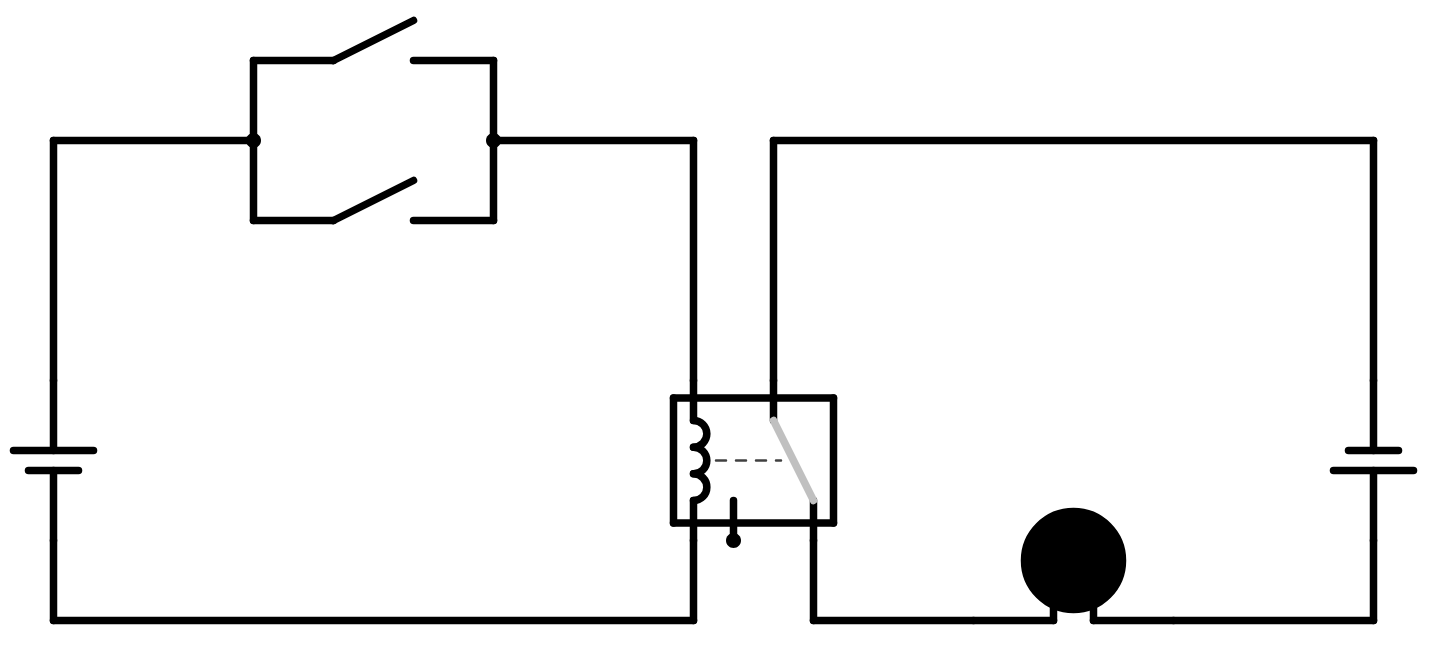
\includegraphics[width=1\textwidth]{./assets/nor-circuit.png}
            \caption{NOR-Schaltung}
        \end{figure}

\end{enumerate}

\section{Aufgabe 5}

Erkl"aren Sie mit eigenen Worten die Bedeutung der Komponenten einer CPU.

\begin{enumerate}[(a)]
    \item \textbf{Steuerwerk} ist eine Einheit der CPU, die den Befehlsdecoder verwendet,
        um eine im Befehlsregister gespeicherte Operation in
        Steuersignale zu entschlüsseln, die den Befehl an andere Einheiten der
        CPU weiterleiten.

    \item \textbf{ALU} ist eine weitere Einheit der CPU, die dazu dient, Berechnungen
        (Addition, Subtraktion, ...) oder logischen Verkn"upfungen (UND, ODER,
        NICHT, ...) durchzuf"uhren.

    \item \textbf{Adresswerk} berechnet Adressen, die zum Abrufen von Daten aus dem
        Hauptspeicher erforderlich sind. Das Adresswerk als eine separate
        Einheit reduziert zus"atzlich die Anzahl der CPU-Zyklen, die für die
        Ausführung verschiedener Maschinenbefehle erforderlich sind, da es
        parallel zum Rest der CPU arbeitet.
\end{enumerate}

\section{Aufgabe 6}

Wozu werden die folgenden Komponenten einer CPU verwendet?

\begin{enumerate}[(a)]
    \item \textbf{Befehlsregister} -- Speichern des aktuell auszuf"uhrenden
            Befehls.
    \item \textbf{Programm-Counter (PC)} -- Speichern der Adresse des n"achsten
        auszuf"uhrenden Befehls.
    \item \textbf{AC-Register} -- temporärer Speicher für die Zwischenergebnisse
        von Berechnungen.
\end{enumerate}

\section{Aufgabe 7}

Es existieren verschiedene Architekturmodelle mit unterschiedlichen
Adressformaten. Schrei- ben Sie f¨ur die nachfolgende Berechnung jeweils ein
Programm unter Verwendung von 3-Adress-, 2-Adress- und 1-Adress-Instruktionen:

\begin{equation*}
    x = (a \cdot b \cdot c) - (d + e)
\end{equation*}

\textbf{L"osung}.

\begin{enumerate}[(a)]
    \item Berechnung unter Verwendung von 1-Adress-Instruktionen:
        \begin{verbatim}
        load a      ; ACC <- a
        mul b       ; ACC <- ACC * b
        mul c       ; ACC <- ACC * c
        sub d       ; ACC <- ACC - d
        sub e       ; ACC <- ACC - e
        store x     ; x <- ACC
        \end{verbatim}
    \item Berechnung unter Verwendung von 2-Adress-Instruktionen:
        \begin{verbatim}
        mul a, b    ; a <- a * b
        mul a, c    ; a <- a * c
        sub a, d    ; a <- a - d
        sub a, e    ; a <- a - e
        \end{verbatim}
    \item Berechnung unter Verwendung von 3-Adress-Instruktionen:
        \begin{verbatim}
        mul a, a, b ; a <- a * b
        mul a, a, c ; a <- a * c
        sub a, a, d ; a <- a - d
        sub a, a, e ; a <- a - e
        \end{verbatim}
\end{enumerate}

\end{document}
